\documentclass[tikz,border=5pt]{standalone}
\usepackage{fontspec}
\setmainfont{Times New Roman}
\usepackage{unicode-math}
\setmathfont{Cambria Math}
\usetikzlibrary{shapes.geometric,positioning,fit,backgrounds,arrows.meta,calc,matrix}

\begin{document}
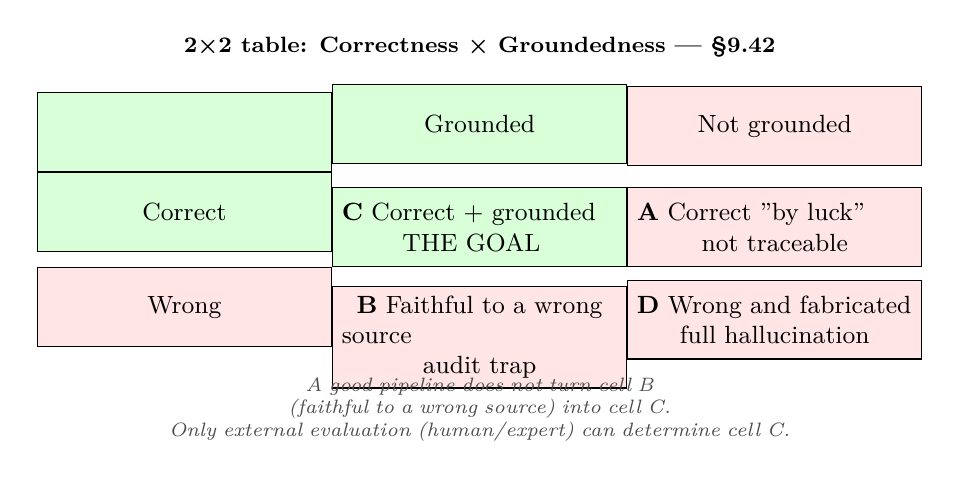
\begin{tikzpicture}
\node[font=\footnotesize\bfseries, align=center] at (0, 2.4) {2×2 table: Correctness × Groundedness --- §9.42};

\matrix (m) [matrix of nodes, nodes={rectangle, draw, align=center, text width=3.5cm, minimum height=1.0cm, font=\small}, column sep=0pt, row sep=0pt] {
  |[fill=green!15]| & |[fill=green!15]| Grounded & |[fill=red!10]| Not grounded \\
  |[fill=green!15]| Correct & |[fill=green!15]| \textbf{C} Correct + grounded \newline ~~~THE GOAL~~~ & |[fill=red!10]| \textbf{A} Correct "by luck" \newline not traceable \\
  |[fill=red!10]| Wrong & |[fill=red!10]| \textbf{B} Faithful to a wrong source \newline audit trap & |[fill=red!10]| \textbf{D} Wrong and fabricated \newline full hallucination \\
};

\node[font=\scriptsize\itshape, text=gray!60!black, align=center, text width=9cm] at (0, -2.2)
  {A good pipeline does not turn cell B (faithful to a wrong source) into cell C.\\Only external evaluation (human/expert) can determine cell C.};

\end{tikzpicture}
\end{document}